%%%%%%%%%%%%%%%%%%%%%%%%%%%%%%%%%%%%%%%%% 
% Beamer Presentation
% LaTeX Template
% Version 1.0 (10/11/12)
% 
% This template has been downloaded from:
% http://www.LaTeXTemplates.com
% 
% License:
% CC BY-NC-SA 3.0 (http://creativecommons.org/licenses/by-nc-sa/3.0/)
% 
%%%%%%%%%%%%%%%%%%%%%%%%%%%%%%%%%%%%%%%%% 

% ----------------------------------------------------------------------------------------
%	PACKAGES AND THEMES
% ----------------------------------------------------------------------------------------

\documentclass{beamer}

\mode<presentation> {

  % The Beamer class comes with a number of default slide themes
  % which change the colors and layouts of slides. Below this is a list
  % of all the themes, uncomment each in turn to see what they look like.

  % \usetheme{default}
  % \usetheme{AnnArbor}
  % \usetheme{Antibes}
  % \usetheme{Bergen}
  % \usetheme{Berkeley}
  % \usetheme{Berlin}
  % \usetheme{Boadilla}
  % \usetheme{CambridgeUS}
  % \usetheme{Copenhagen}
  % \usetheme{Darmstadt}
  % \usetheme{Dresden}
  % \usetheme{Frankfurt}
  % \usetheme{Goettingen}
  \usetheme{Hannover}
  % \usetheme{Ilmenau}
  % \usetheme{JuanLesPins}
  % \usetheme{Luebeck}
  % \usetheme{Madrid}
  % \usetheme{Malmoe}
  % \usetheme{Marburg}
  % \usetheme{Montpellier}
  % \usetheme{PaloAlto}
  % \usetheme{Pittsburgh}
  % \usetheme{Rochester}
  % \usetheme{Singapore}
  % \usetheme{Szeged}
  % \usetheme{Warsaw}

  % As well as themes, the Beamer class has a number of color themes
  % for any slide theme. Uncomment each of these in turn to see how it
  % changes the colors of your current slide theme.

  % \usecolortheme{albatross}
  % \usecolortheme{beaver}
  % \usecolortheme{beetle}
  % \usecolortheme{crane}
  % \usecolortheme{dolphin}
  % \usecolortheme{dove}
  % \usecolortheme{fly}
  % \usecolortheme{lily}
  \usecolortheme{orchid}
  % \usecolortheme{rose}
  % \usecolortheme{seagull}
  % \usecolortheme{seahorse}
  % \usecolortheme{whale}
  % \usecolortheme{wolverine}

  % \setbeamertemplate{footline} % To remove the footer line in all slides uncomment this line
  % \setbeamertemplate{footline}[page number] % To replace the footer line in all slides with a simple slide count uncomment this line

  % \setbeamertemplate{navigation symbols}{} % To remove the navigation symbols from the bottom of all slides uncomment this line
}

\usepackage{graphicx} % Allows including images
\usepackage{multirow}
\usepackage{booktabs} % Allows the use of \toprule, \midrule and \bottomrule in tables
\graphicspath{ {images/} }

% ----------------------------------------------------------------------------------------
%	TITLE PAGE
% ----------------------------------------------------------------------------------------

\title[IC Verification Automation]{IC Verification Automation} % The short title appears at the bottom of every slide, the full title is only on the title page

\author{Guanyu Yi} % Your name
\institute[cmos] % Your institution as it will appear on the bottom of every slide, may be shorthand to save space
{
  % Spreadtrum Communications, Inc. \\ % Your institution for the title page
  \medskip
  \textit{gary3511@gmail.com} % Your email address
}
\date{April 5, 2016} % Date, can be changed to a custom date

\begin{document}

\begin{frame}
  \titlepage % Print the title page as the first slide
\end{frame}

\begin{frame}
  \tableofcontents % Throughout your presentation, if you choose to use \section{} and \subsection{} commands, these will automatically be printed on this slide as an overview of your presentation
\end{frame}

% ----------------------------------------------------------------------------------------
%	PRESENTATION SLIDES
% ----------------------------------------------------------------------------------------

% ------------------------------------------------
\section{Verification Trends} % Sections can be created in order to organize your presentation into discrete blocks, all sections and subsections are automatically printed in the table of contents as an overview of the talk
% ------------------------------------------------

% \subsection{Subsection Example} % A subsection can be created just before a set of slides with a common theme to further break down your presentation into chunks

\begin{frame}

  \textbf{Important verification}
  \begin{enumerate}
  \item More average verification time consumption
  \item More projects spending a lot of time in verification
  \end{enumerate}
  \begin{figure}
    \centering
    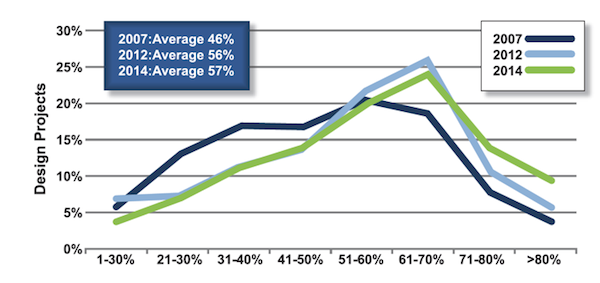
\includegraphics[width=0.9\linewidth]{wilson1}
    \caption{Percentage of IC project time spent in verification}
  \end{figure}

\end{frame}

\begin{frame}

  \textbf{Important verification Time}
  \begin{enumerate}
  \item Debug consumes a lot of time
  \item Relationship with TB building and SIM running
  \end{enumerate}
  \begin{figure}
    \centering
    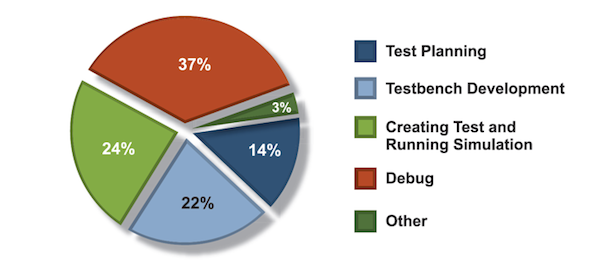
\includegraphics[width=0.9\linewidth]{wilson5}
    \caption{Where IC verification engineers spend their time}
  \end{figure}

\end{frame}

% ------------------------------------------------
\section{Efficiency Solutions}
% ------------------------------------------------

\begin{frame}
  \begin{block}{Saving Verification Time}
    \begin{enumerate}
    \item TB configuration
    \item DUT configuration
    \item EDA tools optimization
    \end{enumerate}
  \end{block}
\end{frame}

\begin{frame}
  \begin{columns}[c] % The "c" option specifies centered vertical alignment while the "t" option is used for top vertical alignment

    \column{.45\textwidth} % Left column and width
    \textbf{TB configuration}
    \begin{enumerate}
    \item UVM -- Universal Verification Methodology
    \item Coverage driven verification flow
    \item Reusable configurable environment
    \item Ready-to-use components
    \end{enumerate}

    \column{.5\textwidth} % Right column and width
    \begin{figure}
      \centering
      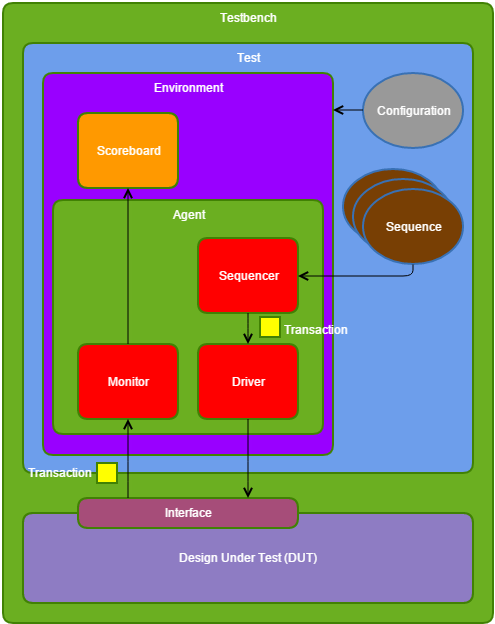
\includegraphics[width=0.9\linewidth]{uvm_arch}
      \caption{A typical UVM arch}
    \end{figure}

  \end{columns}
\end{frame}

\begin{frame}
  \begin{columns}[c] % The "c" option specifies centered vertical alignment while the "t" option is used for top vertical alignment

    \column{.45\textwidth} % Left column and width
    \textbf{DUT configuration}
    \begin{enumerate}
    \item DUT splitting
    \item Case specified configuration
    \item Flexible and Customized extension
    \end{enumerate}

    \column{.5\textwidth} % Right column and width
    \begin{figure}
      \centering
      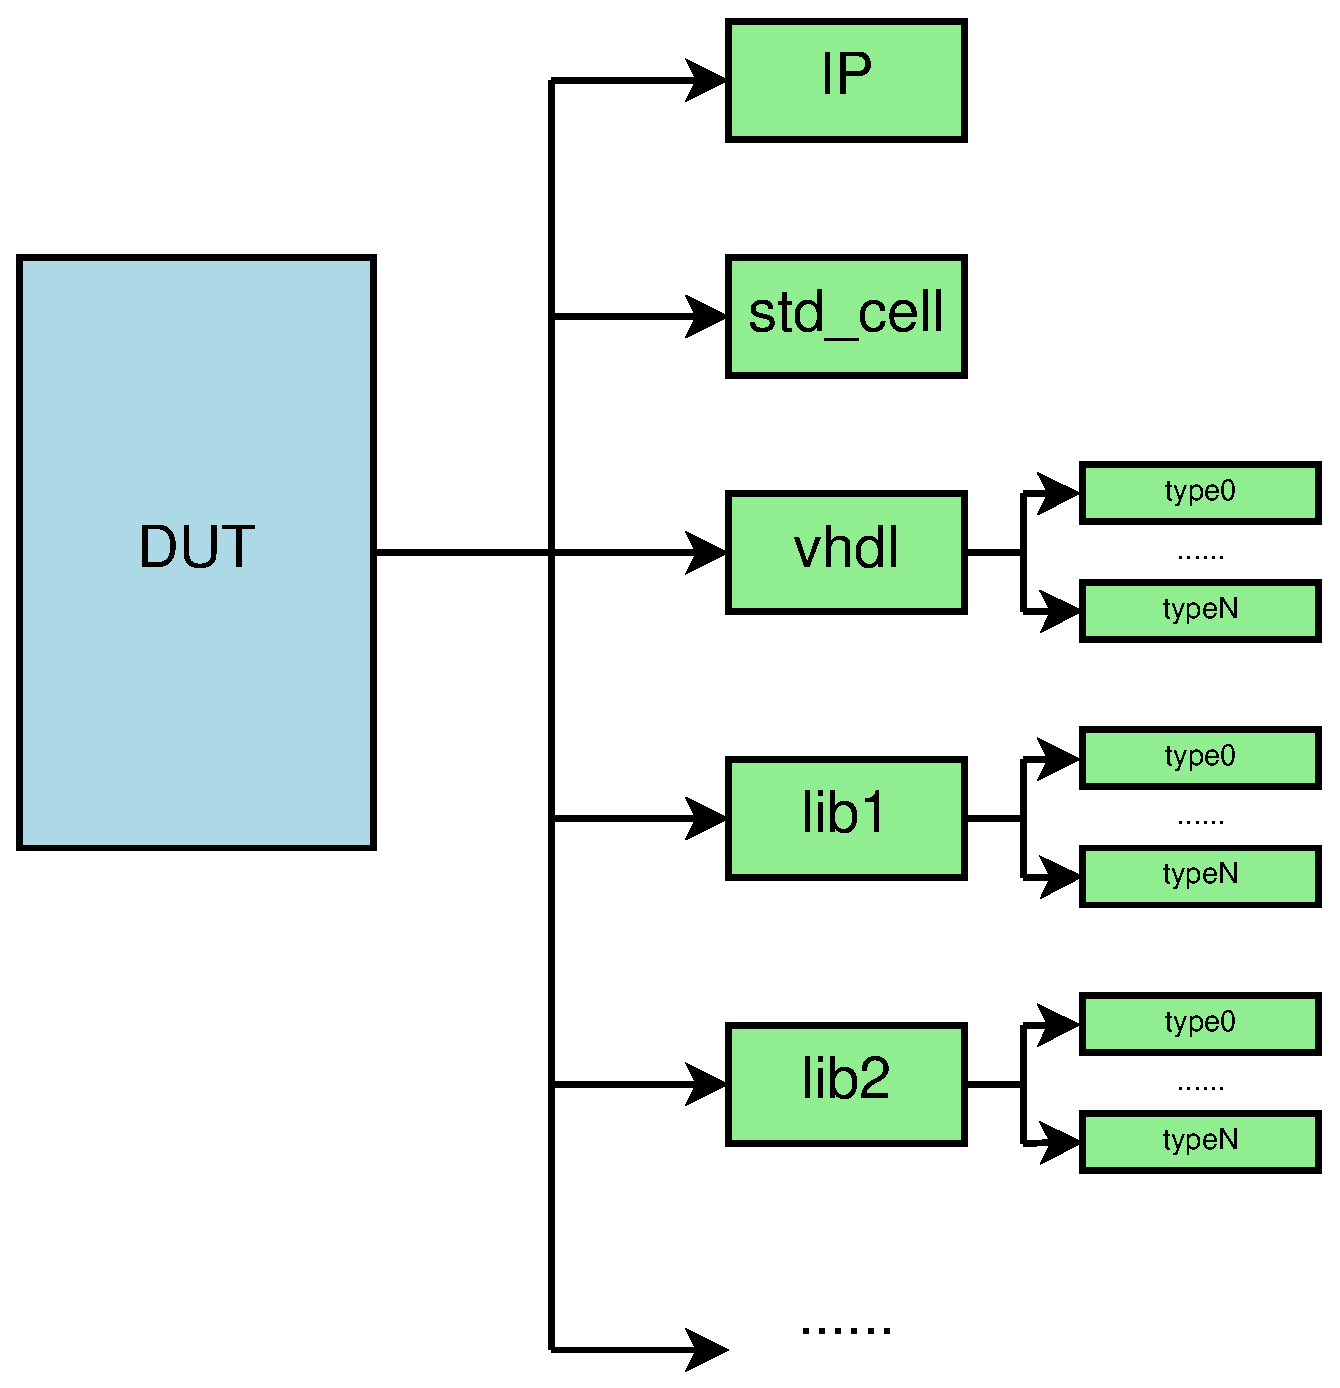
\includegraphics[width=0.9\linewidth]{dut_split}
      \caption{Configurable DUT arch}
    \end{figure}

  \end{columns}
\end{frame}

\begin{frame}
  \begin{columns}[c] % The "c" option specifies centered vertical alignment while the "t" option is used for top vertical alignment

    \column{.45\textwidth} % Left column and width
    \textbf{EDA tools optimization}
    \begin{enumerate}
    \item Cadence -- MSIE
    \item Synopsys -- PIP
    \item Time-space trade-off
    \item Saving compilation and elaboration time
    \end{enumerate}

    \column{.5\textwidth} % Right column and width
    \begin{figure}
      \centering
      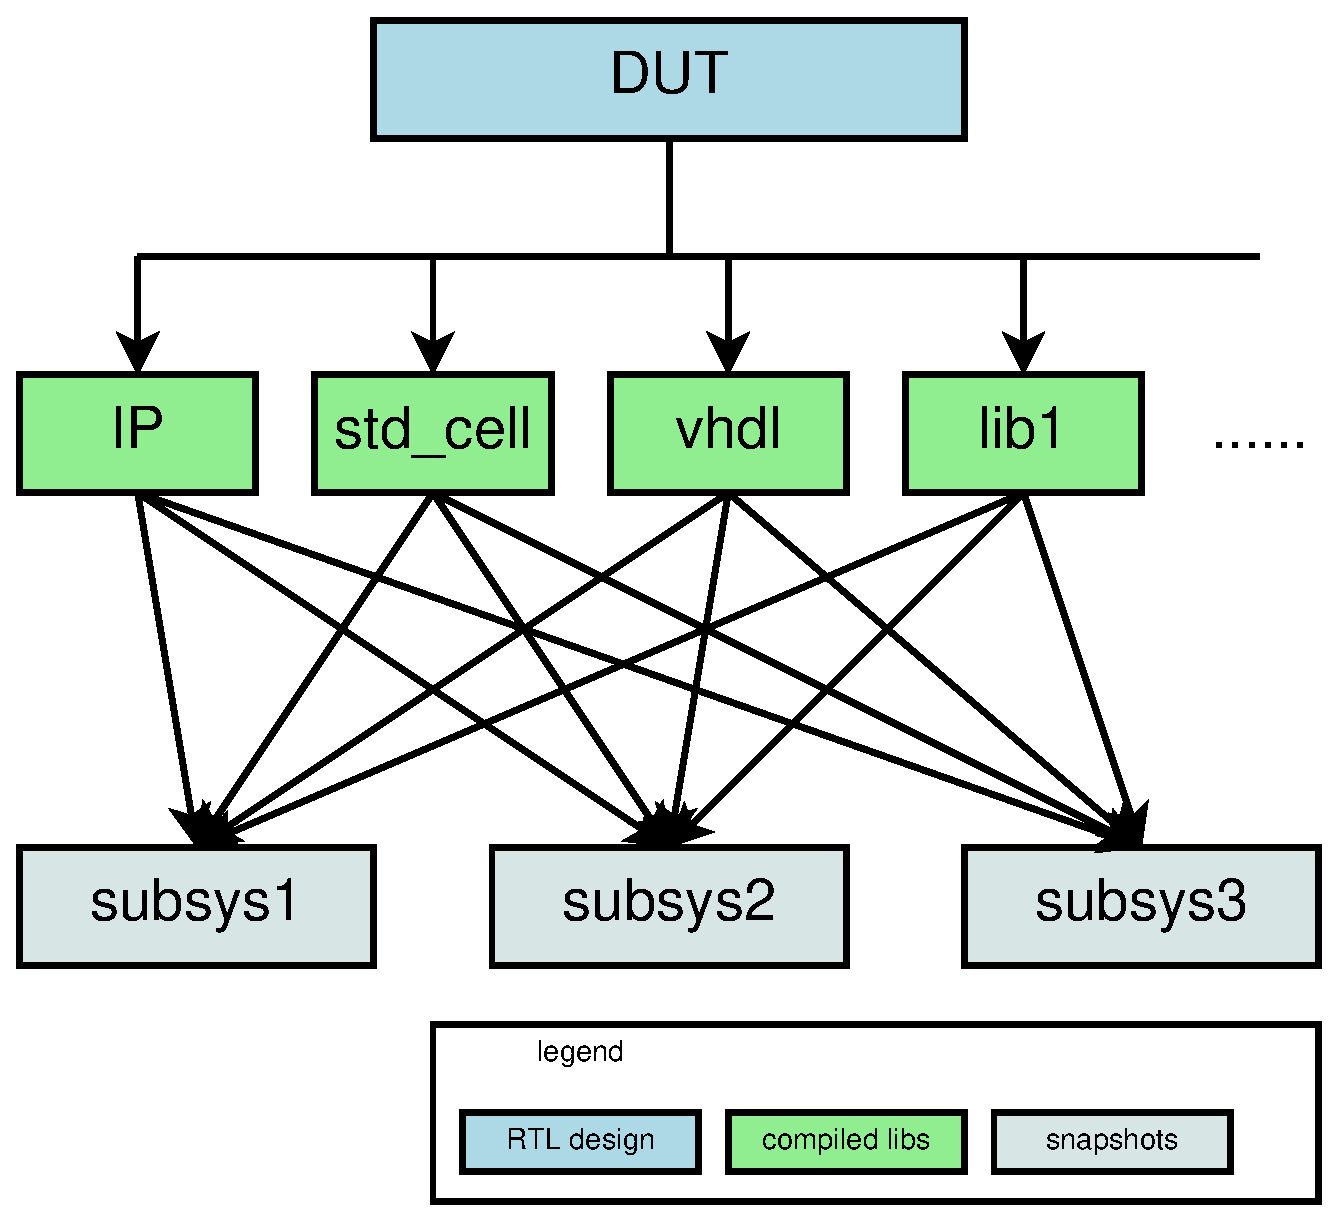
\includegraphics[width=0.9\linewidth]{pm_mapping}
      \caption{MSIE/PIP flow arch}
    \end{figure}

  \end{columns}
\end{frame}

\begin{frame}
  \begin{table}
    \centering
    \begin{tabular}{lll}
      \toprule
      \textbf{Steps} & \textbf{Time New} & \textbf{Time Legacy} \\
      \midrule
      pre comp & 1min 12sec* & \multirow{5}{*}{23min 22sec} \\
      \cline{1-2}
      MSIE elab & 2min 23sec* & \\
      \cline{1-2}
      href gen & 2min 29sec* & \\
      \cline{1-2}
      re elab & 2min 29sec* & \\
      \cline{1-2}
      inc elab & 2min 16sec & \\
      \hline
      total & 2min 16sec & 23min 22sec \\
      \bottomrule
      \multicolumn{3}{l}{\footnotesize{* the time marked with star is shared by every case}}
    \end{tabular}
    \caption{Time consumption comparison table}
  \end{table}
\end{frame}

% ------------------------------------------------
\section{Verification Automation}
% ------------------------------------------------

\begin{frame}
  \begin{figure}
    \centering
    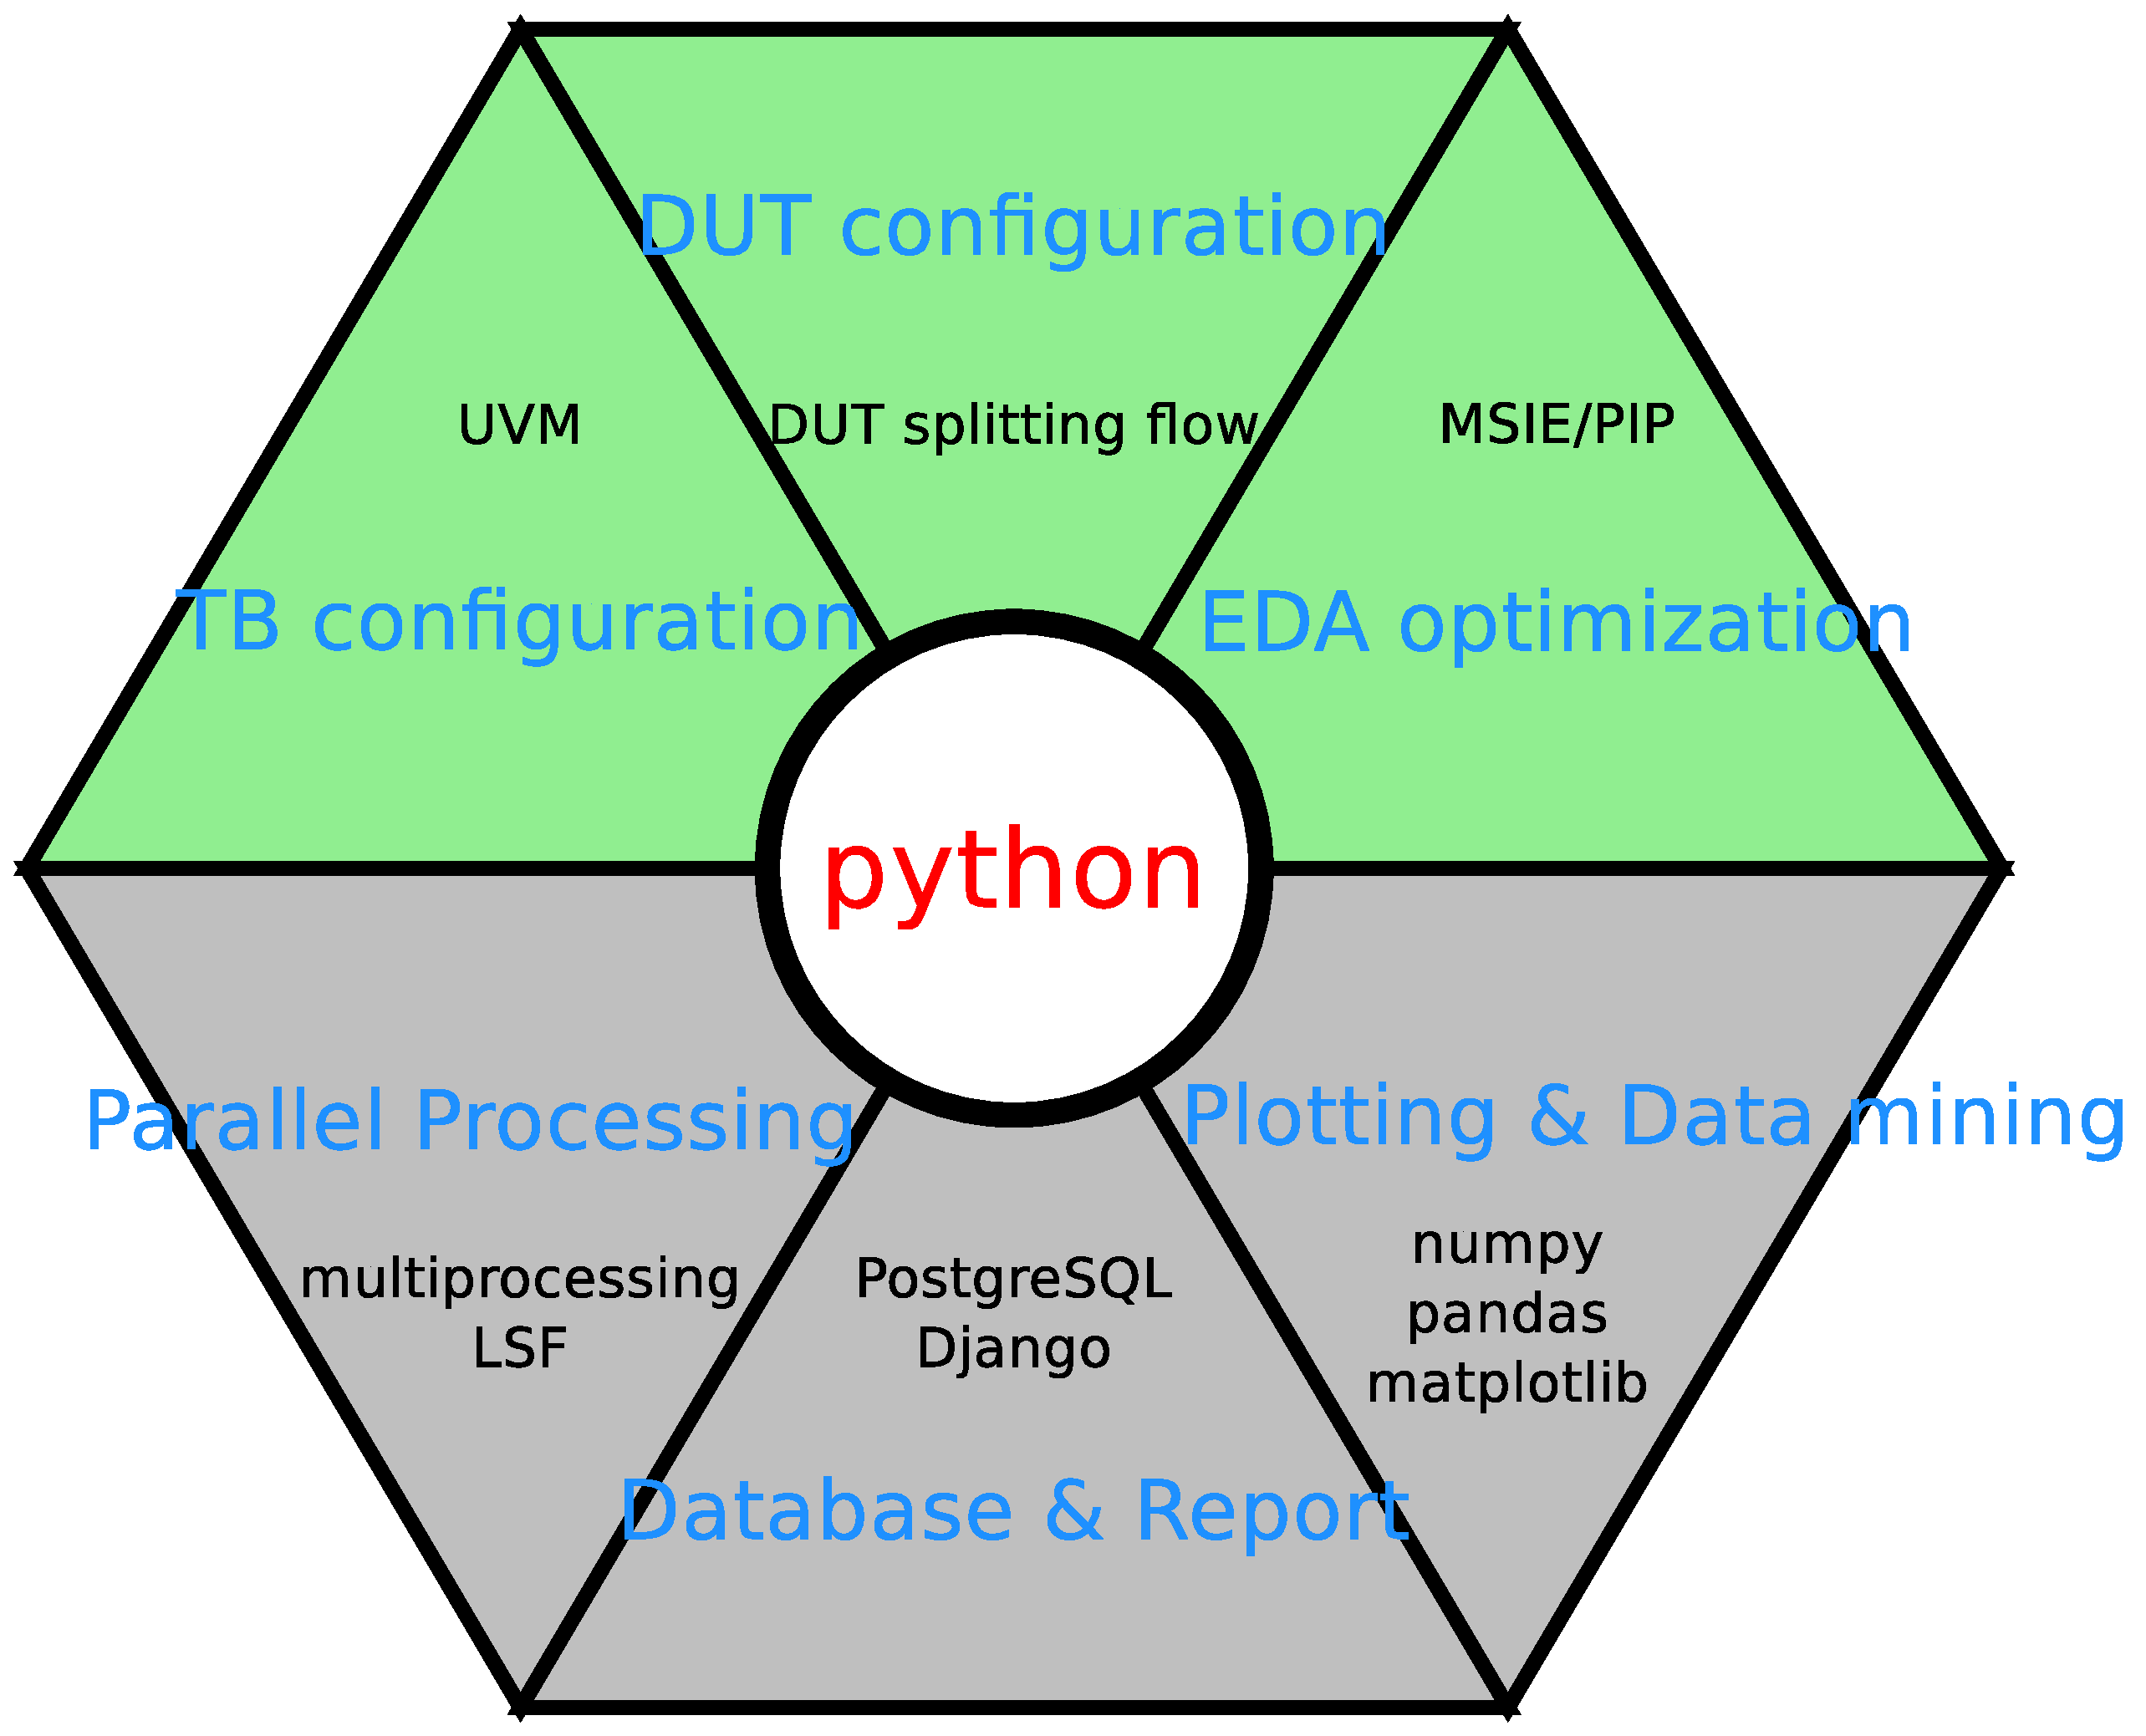
\includegraphics[width=0.9\linewidth]{verification_automation}
    \caption{Verification automation architecture}
  \end{figure}
\end{frame}

\begin{frame}
  \Huge{\centerline{Thank you!}}
\end{frame}

% ----------------------------------------------------------------------------------------

\end{document}
%%% Local Variables:
%%% mode: latex
%%% TeX-master: t
%%% End:
